% !TEX encoding = MacOSRoman
\documentclass{beamer}
\usepackage[utf8]{inputenc}
\usepackage{amsfonts}
\usepackage{textcomp}
\usepackage{listings}
\usepackage{graphicx}
\usepackage{numprint}
\usepackage{subfigure}
\usepackage{tikz}
\usetikzlibrary{shapes.geometric, arrows}
\usepackage{setspace}
\usepackage{termlist}
\usepackage{amsmath}
\usepackage{amsmath}
\usepackage{amssymb}
\usepackage{amsthm}
\usepackage{bm} 
 
\newcommand{\samelineand}{\qquad} 
 
%Information to be included in the title page:
\title{Analysis of time delay data and clock drift in a network of seismic monitors}
\author{Jordi Anguera \inst{1} \and 
Leevi Annala \inst{2} \and 
Stefan Dimitrijevic \inst{3} \and 
Patricia Pauli \inst{4} \and 
Liisa-Ida Sorsa \inst{5} \and 
Dimitar Trendafilov \inst{6} \and 
Christophe Pickard \inst{7}}

\institute[XLIM]{\inst{1} Autonomous University of Barcelona, Spain \samelineand 
	\inst{2}University of Jyväskylä, Finland \and 
	\inst{3} University of Novi Sad, Serbia \samelineand 
	\inst{4}Technical University of Darmstadt, Germany \and 
	\inst{5}Tampere University of Technology, Finland  \and 
	\inst{6} University of Sofia ''St. Kliment Ohridski'', Bulgaria \and 
	\inst{7} University of Grenoble Alpes and Grenoble INP, France}
\date{ECMI Modelling Week, 21 July 2018} 
 
\begin{document}
 
\frame{\titlepage}

\makeatletter
\makeatother

\section{Problem statement}
\begin{frame}
\frametitle{Problem statement}
\begin{itemize}
\item Seismic monitoring is used to study the behaviour and composition of the underground floor
\item Continuous synchronization to the Global Positioning System for accurate timing is not possible 
\item The instruments' clocks deviate in time causing lack of accuracy in the measurements
\item A reliable method to correct for the time deviation is required
\item Real data collected from a network of seismic monitors over time is analyzed
\item The problem is to discern the time drift of the clock in each monitor from noise and actual data
\end{itemize}
\end{frame}

\section{Data}

\begin{frame}
\frametitle{The network of seismic monitors}
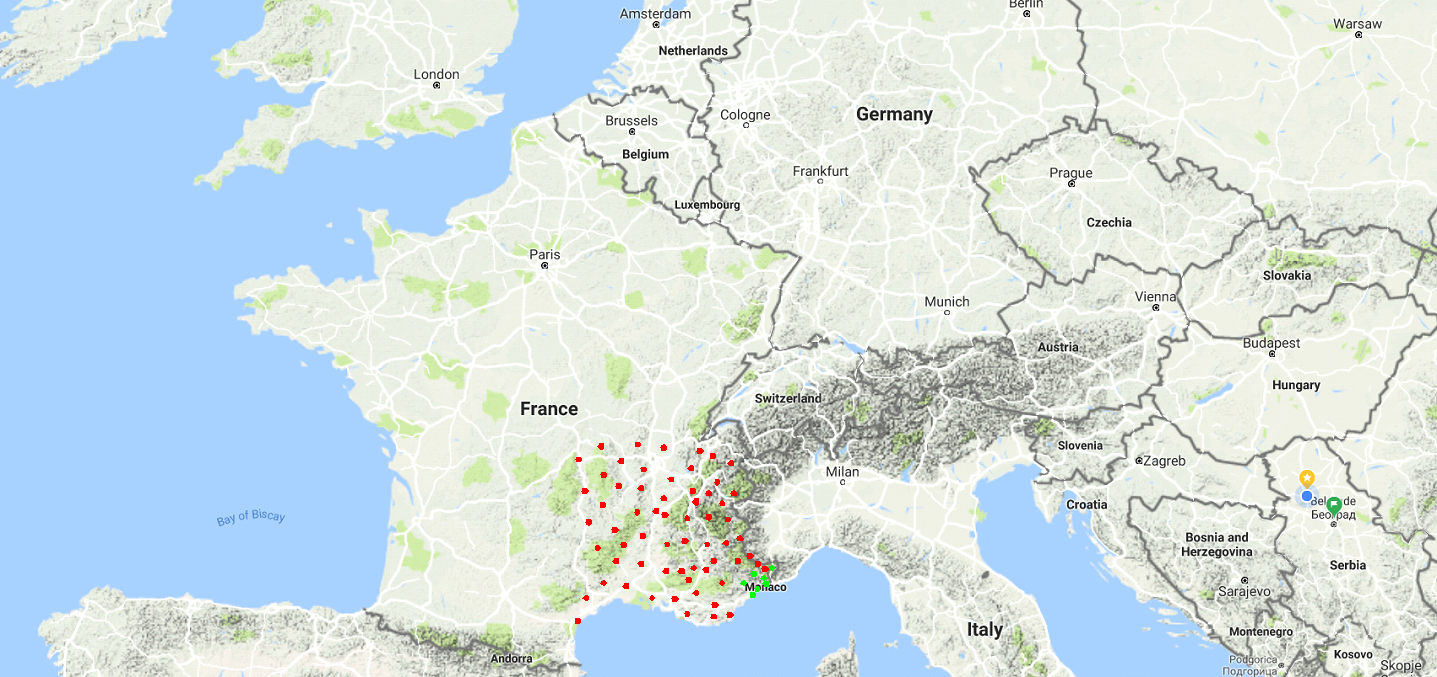
\includegraphics[width=\textwidth]{InitialStationSet.png}
\end{frame}

\begin{frame}
\frametitle{The network of seismic monitors}
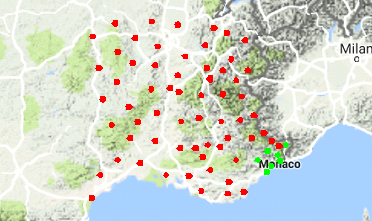
\includegraphics[width=\textwidth]{InitialStationSet_zoom.png}
\end{frame}

\begin{frame}
\frametitle{Numbers of working stations and connections to stations during one year}

\begin{itemize}
\item The network consists of 73 seismic monitors
\item Not all monitors work at all times
\item If two monitors are working simultaneously, they are connected
\item Connections are undirected
\end{itemize}

\begin{columns}
\column{0.5\textwidth}
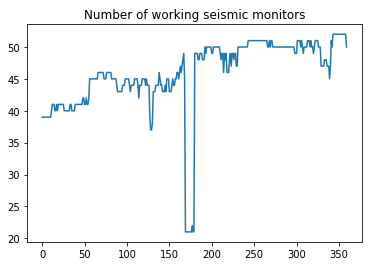
\includegraphics[width=\textwidth]{working_monitors.png}

\column{0.5\textwidth}
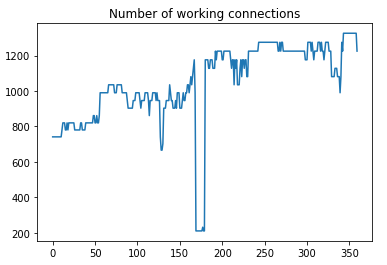
\includegraphics[width=\textwidth]{working_connections.png}
\end{columns}
\end{frame}

\begin{frame}
\frametitle{Time-delay signal characteristics}
\begin{itemize}
\item Data recorded in one second intervals
\item Time-delay cross-correlation in one-hour intervals
\item Tracing time-delays recorded by one station over a year
\item Time delays are computed in both directions (from A $\rightarrow$ B and B $\rightarrow$ A) and are opposite numbers
\end{itemize}

\begin{columns}
\column{0.5\textwidth}
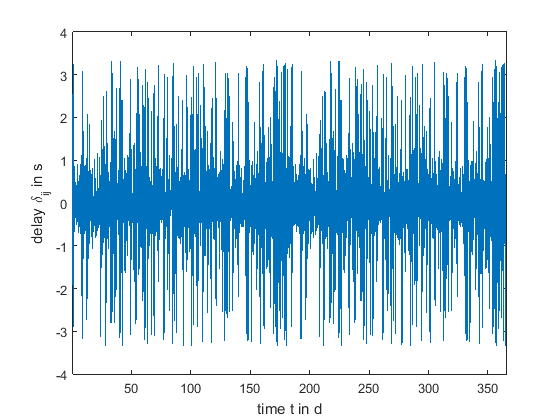
\includegraphics[width=\textwidth]{delayevolutionovertimeforonestation2.png}

\column{0.5\textwidth}
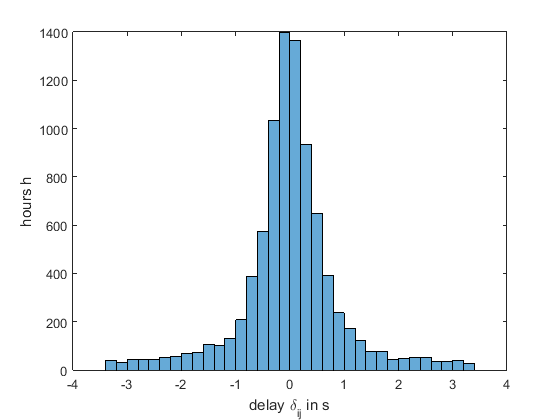
\includegraphics[width=\textwidth]{delayevolutionovertimeforonestation.png}
\end{columns}
\end{frame}

\begin{frame}
\frametitle{Histograms showing time delays recorded by all active stations over 24 hours}
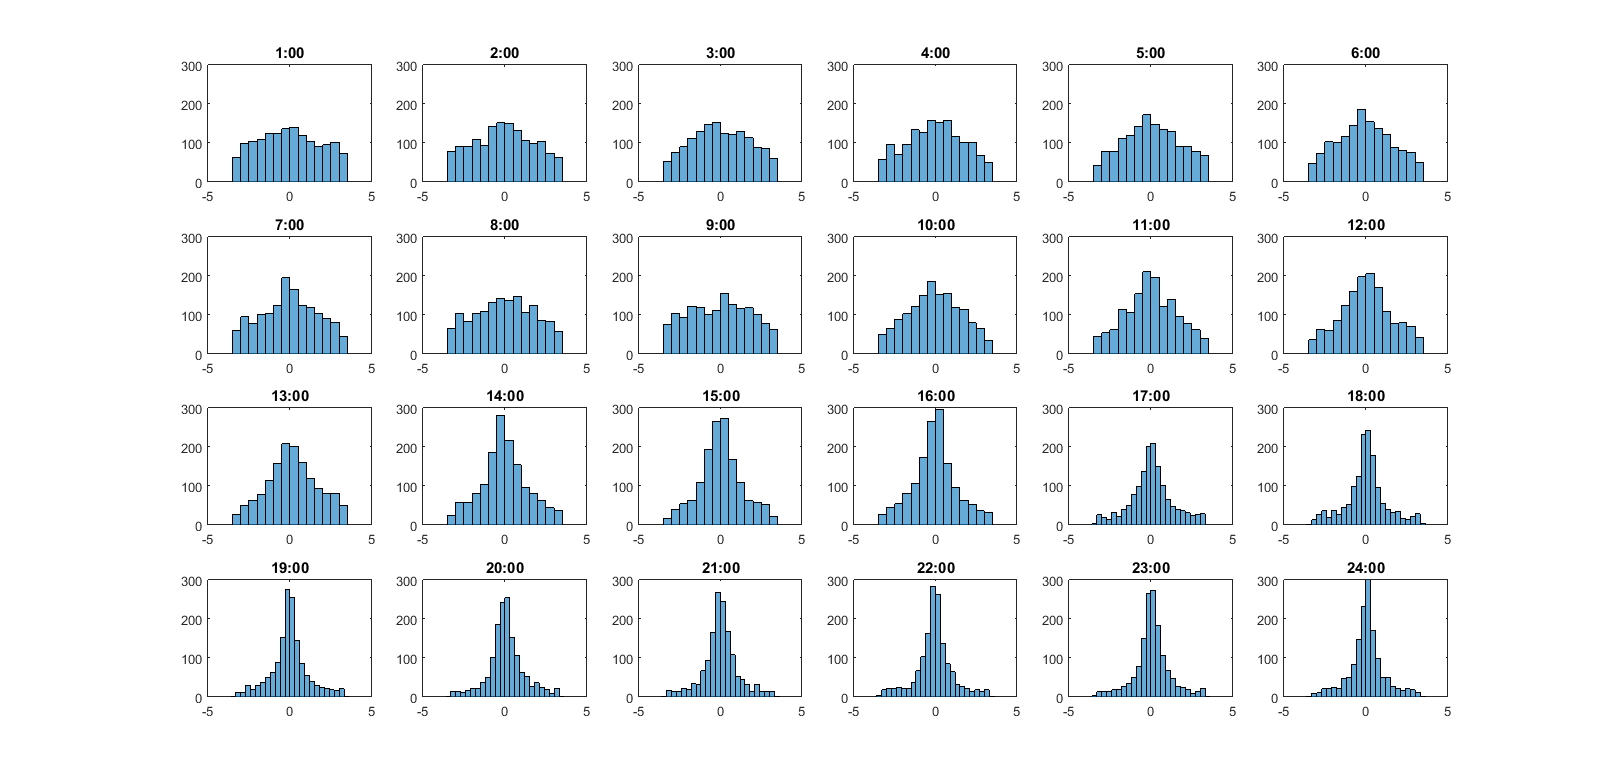
\includegraphics[width=\textwidth]{hourlydelaydistributionoverallstationsforoneday.png}
\end{frame}

\begin{frame}
\frametitle{Comparison of time delay of the furthest and the closest station pairs}
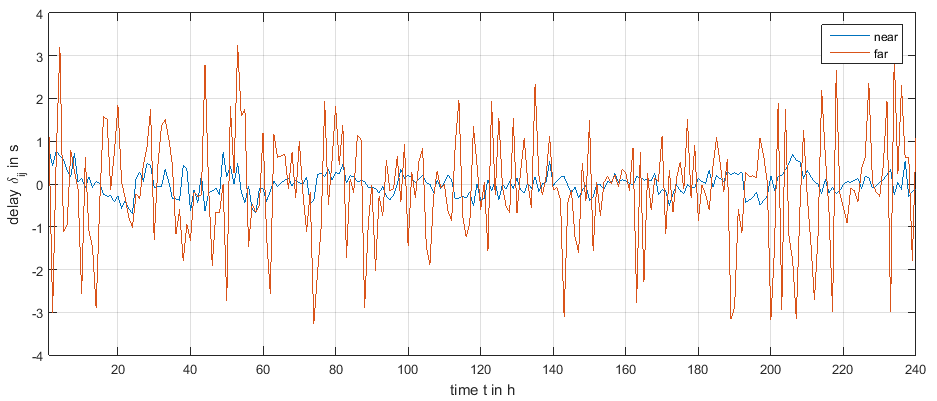
\includegraphics[width=\textwidth]{Comparisondelayoverrandomdayoffarestandclosestlinks.png}

\begin{itemize}
\item Time delays are smaller between stations which are close to each other
\item The non-linear trace of the data is thought to be caused by the station's non-ideal clock (clock drift)
\end{itemize}
\end{frame}

\section{Model}

\begin{frame}
\frametitle{Clock drift and errors in the data}
\begin{itemize}
\item The measurements $\bm{\hat{\delta}}$ of time delays between stations
\end{itemize}
\begin{equation}
\bm{\hat{\delta}}  = \bm{\delta} + \bm{\varepsilon}.
\label{eq:model}
\end{equation}

\begin{itemize}
\item The error $\varepsilon_{ij}$ is error in time delay between stations $i$ and $j$
\end{itemize}

\begin{equation}
\varepsilon_{ij} = | \Delta_i - \Delta_j | + e_{ij},
\end{equation}
\quad \quad $\Delta_i$ is the clock drift of station $i$

\quad \quad $e_{ij}$ includes other measurement errors
\end{frame}


\begin{frame}
\frametitle{Graph approach to model the data}
\begin{itemize}
\item A weighted graph $\mathcal{G} = (\mathcal{V}, \mathcal{E}, \bm{\hat{\delta}}_t)$
\item Weighted adjacency matrix of time delays $ \bm{\hat{\delta}}_t)$ is symmetric with $\delta_{ii} = 0$
\item Values $\hat{\delta}_{ij}$ are normalized to $[0,1]$
\item A normalized (to $[0,1]$) distance measure was selected as graph metrics $K_m$
\begin{equation}
K_m = f_m (r_i)= \sum_j{r_{ij}}.  
\end{equation}
\end{itemize}
\end{frame}


\begin{frame}
\frametitle{Signal denoising}
\begin{itemize}
\item We specify a cost function $c(\bm{\hat{\delta}})$ measuring the deviation from the observed weight matrix's metrics $f_m(\bm{\hat{\delta}})$ to the estimates of the distance metrics $K_m$


\begin{equation}
c(\bm{\hat{\delta}}) = \sum_m e_m^2(\bm{\hat{\delta}}) = \sum_m(f_m(\bm{\hat{\delta}})-K_m)^2
\end{equation}

\item Error is minimized with gradient descent updates on $\bm{\hat{\delta}}$: 

\begin{equation}
\bm{\hat{\delta}}^{(t+1)} = \bm{\hat{\delta}}^t-\mu\sum_m e_m(\bm{\hat{\delta}}^t)\frac{df_m(\bm{\hat{\delta}}^t)}{d\bm{\hat{\delta}}^t},
\label{eq:updates}
\end{equation}
\end{itemize}
\end{frame}

\begin{frame}
\frametitle{Exctracting clock drift from noise}
\begin{itemize}
\item The noise $\varepsilon_{ij}$ between each pair of two stations is modelled with
\begin{equation}
\varepsilon_{ij} = | \Delta_i - \Delta_j | + e_{ij},
\end{equation}
\quad \quad in which $\Delta_i$ and $\Delta_j$ are the clock drifts of stations $i, j$
\quad \quad $e_{ij}$ accounts for all other noise in the system

\item A polynomial curve is fitted to the extracted noise to trace clock drift
\end{itemize}
\end{frame}

\begin{frame}%[shrink=20]
\frametitle{Solvin individual clock drifts (1/2)}
\begin{itemize}
\item We have overdetermined inverse problem of the form
\begin{equation}
Gm = s
\end{equation}

\footnotesize
\begin{equation*}
\begin{bmatrix}
1 & -1 & 0 & 0 & \dots  & 0 \\
1 & 0 & -1 & 0 & \dots  & 0 \\
1 &  0  & 0 & -1 & \dots   & 0 \\
\vdots & \vdots & \vdots  & \vdots & \ddots & \vdots \\
1 &  0  & 0 & 0 & \dots & -1 \\
0 &  1  & -1 & 0 & \dots & 0 \\
0 & 1 & 0 & -1 & \dots & 0 \\
0 & 1 & 0 & 0 & \ddots & 0 \\
\hdotsfor{6} \\
0 & 0 & \dots & 0& 1 & -1
\end{bmatrix}
 \begin{bmatrix}
\Delta_1 \\ \Delta_2 \\ \Delta_3 \\ \Delta_4 \\ \vdots \\ \Delta_k \\ \vdots \\ \Delta_{n-1} \\ \Delta_n
\end{bmatrix}
 = 
 \begin{bmatrix}
 \Delta_1 - \Delta_2 \\ \Delta_1-\Delta_3 \\ \Delta_1-\Delta_4 \\ \vdots \\ \Delta_1 - \Delta_{n} \\ \Delta_2- \Delta_3 \\ \Delta_2 - \Delta_4 \\ \vdots  \\ \Delta_2-\Delta_k \\ \vdots \\ \Delta_{n-1} - \Delta_n
 \end{bmatrix}
= 
\begin{bmatrix}
\Delta_{12} \\ \Delta_{13} \\ \Delta_{14} \\ \vdots \\ \Delta_{1n} \\ \Delta_{23} \\ \Delta_{24} \\ \vdots \\ \Delta_{2k} \\ \vdots \\ \Delta_{(n-1)n}
\end{bmatrix} 
\end{equation*}
\normalsize

\item Matrix $G$ rank is $n-1$
\end{itemize}
\end{frame}

\begin{frame}
\frametitle{Solving individual clock drifts 1/2}
\begin{itemize}
\item Ordinary least squares regression
\begin{equation}
\| \mathbf{Gm}-\mathbf{s} \|_2^2.
\label{eq:leastsquares}
\end{equation}

\item Tikhonov regularization is employed
\begin{equation}
\| \mathbf{Gm}-\mathbf{s} \|_2^2 + \| \bm{\Gamma}\mathbf{m} \|_2^2, 
\label{eq:tikhonov}
\end{equation}
\quad \quad for some suitable Tikhonov matrix $\bm{\Gamma} = \alpha\mathbf{I}$
\item The explicit solution is hence given by
\begin{equation}
\hat{\mathbf{s}} = (\mathbf{G}^T\mathbf{G} + \bm{\Gamma}^T\bm{\Gamma})^{-1}\mathbf{G}^T\mathbf{m}.  
\end{equation}

\end{itemize}

\end{frame}

\section{Results}
\begin{frame}
\frametitle{Results}
\end{frame}

\section{Conclusion}
 \begin{frame}
\frametitle{Conclusion}
\end{frame}
 
\end{document}

